\documentclass[12pt,letterpaper,twoside]{article}
\usepackage{amsmath,amssymb,amsfonts}
\usepackage{graphicx}
\usepackage{tikz}
\usepackage{pgfplots}
\pgfplotsset{compat=1.17}
\usepackage{xcolor}
\usepackage{hyperref}
\usepackage{cleveref}
\usepackage{booktabs}
\usepackage{caption}
\usepackage{subcaption}
\usepackage{wrapfig}
\usepackage{nicefrac}
\usepackage{minted}
\usepackage{geometry}
\geometry{margin=1in, top=0.75in, bottom=0.75in}

% Colors for thermodynamic gating visualization
\definecolor{thermoblue}{RGB}{31, 119, 180}
\definecolor{thermored}{RGB}{214, 39, 40}
\definecolor{thermogreen}{RGB}{44, 160, 44}
\definecolor{thermopurple}{RGB}{148, 103, 189}
\definecolor{thermoorange}{RGB}{255, 127, 14}
\definecolor{thermoteal}{RGB}{44, 174, 175}
\definecolor{thermoyellow}{RGB}{188, 189, 34}

% TikZ libraries
\usetikzlibrary{decorations.pathmorphing,shapes.geometric,calc,positioning,arrows.meta,patterns}

% Title and Author
\title{\textbf{Thermodynamic Gating: Dissipation-Controlled Memory in Geodesic Flow Networks}}

\author{Joaquin Stürtz}

\date{January 24, 2026}

% Header
\pagestyle{myheadings}
\markright{Thermodynamic Gating}
\lhead{Manifold Learning Research}
\rhead{\thepage}

% Theorem-like environments
\newtheorem{definition}{Definition}[section]
\newtheorem{theorem}{Theorem}[section]
\newtheorem{Lemma}{Lemma}[section]
\newtheorem{example}{Example}[section]
\newtheorem{remarque}{Remark}[section]
\newtheorem{prop}{Proposition}[section]
\newtheorem{corol}{Corollary}[section]

% Macros for frequently used notation
\newcommand{\M}{\mathcal{M}}
\newcommand{\R}{\mathbb{R}}
\newcommand{\T}{\mathbb{T}}
\newcommand{\Sph}{\mathbb{S}}
\newcommand{\diff}{\mathrm{d}}
\newcommand{\grad}{\nabla}
\newcommand{\divop}{\nabla\!\cdot\!}
\DeclareMathOperator{\Tr}{Tr}
\DeclareMathOperator{\diag}{diag}
\DeclareMathOperator{\sech}{sech}
\DeclareMathOperator{\erf}{erf}

\begin{document}

\maketitle
\thispagestyle{empty}

\vspace{0.5cm}

\begin{abstract}
Hamiltonian latent dynamics preserve phase-space volume, enabling long-horizon persistence of information. Yet strict conservation impedes contextual switching: a purely conservative system cannot relax into new semantic attractors without oscillation. We introduce \textbf{Thermodynamic Gating}, a mechanism that couples Hamiltonian geodesic flow to a learned dissipative field and a dynamic time gate. A state- and input-dependent friction coefficient $\mu(x,u)$ implements selective irreversibility (the ``clutch''), while a curvature-informed gate scales the effective time step $\Delta t_{\text{eff}} = g(x)\,\Delta t$. The result is a conformal-symplectic update that supports both persistent memory (coasting) and decisive rewriting (damping), verified in the reference implementation by an implicit friction Leapfrog scheme and toroidal topology features for periodic computation.
\end{abstract}

\vspace{0.5cm}
\hrule
\vspace{0.5cm}

\tableofcontents
\newpage

\section{Motivation: Conservation, Updating, and Selective Irreversibility}

The fundamental tension in sequence modeling is between \textbf{memory} and \textbf{adaptability}:

\begin{itemize}
\item \textbf{Conservation} preserves gradients and memory but resists settling; information persists indefinitely, even when it should be updated.
\item \textbf{Naive damping} destroys long-horizon stability; aggressive dissipation eliminates the very gradients that enable learning.
\end{itemize}

Intelligent behavior requires switching between two regimes:

\begin{enumerate}
\item \textbf{Isolated Regime} (conservative flow): Information is preserved, gradients flow backward through time, and the system ``coasts'' on accumulated momentum.
\item \textbf{Open Regime} (entropy-producing update): Information is selectively erased, dissipation produces the entropy required for state transitions, and the system ``relaxes'' into new attractors.
\end{enumerate}

Thermodynamic Gating provides a physical basis for this switching: dissipation is produced only where and when information must be rewritten. This mirrors Landauer's principle---erasure requires heat dissipation---and connects neural computation to thermodynamic laws.

\begin{figure}[htbp]
\centering
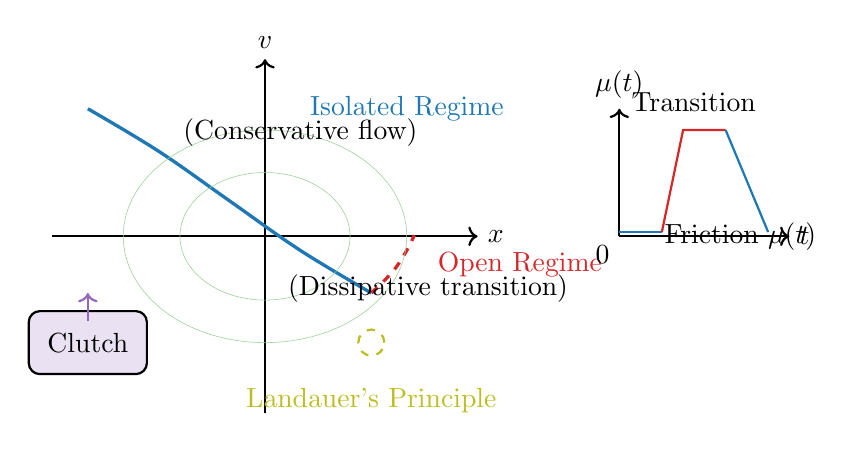
\begin{tikzpicture}[scale=0.9]
    % Phase space diagram showing regime transitions
    \draw[->, thick] (-3, 0) -- (3, 0) node[right] {$x$};
    \draw[->, thick] (0, -2.5) -- (0, 2.5) node[above] {$v$};
    
    % Conservative trajectory (coasting)
    \draw[thermoblue, very thick] 
        plot[smooth,tension=0.6] coordinates {
            (-2.5, 1.8) (-1.5, 1.2) (-0.5, 0.5) (0.5, -0.2) (1.5, -0.8)
        };
    
    % Dissipative transition (damping)
    \draw[thermored, very thick, dashed] 
        plot[smooth,tension=0.7] coordinates {
            (1.5, -0.8) (1.8, -0.5) (2.0, -0.2) (2.1, 0) (2.1, 0)
        };
    
    % Energy contours
    \draw[thermogreen!50, very thin] ellipse (2 and 1.5);
    \draw[thermogreen!50, very thin] ellipse (1.2 and 0.9);
    
    % Regime annotations
    \node[thermoblue, right] at (0.5, 1.8) {Isolated Regime};
    \node[below] at (0.5, 1.8) {(Conservative flow)};
    
    \node[thermored, right] at (2.3, -0.4) {Open Regime};
    \node[below] at (2.3, -0.4) {(Dissipative transition)};
    
    % Clutch visualization
    \node[draw, rectangle, rounded corners, fill=thermopurple!20, thick, minimum width=1.5cm, minimum height=0.8cm] at (-2.5, -1.5) {Clutch};
    \draw[->, thick, thermopurple] (-2.5, -1.2) -- (-2.5, -0.8);
    
    % Landauer's principle annotation
    \node[draw, ellipse, dashed, thermoyellow, thick] at (1.5, -1.5) {};
    \node[thermoyellow, below] at (1.5, -2) {Landauer's Principle};
    
    % Friction coefficient visualization
    \begin{scope}[shift={(5, 0)}, scale=0.6]
        \draw[->, thick] (0, 0) -- (4, 0) node[right] {$t$};
        \draw[->, thick] (0, 0) -- (0, 3) node[above] {$\mu(t)$};
        
        \draw[thermoblue, thick] (0, 0.1) -- (1, 0.1) -- (1, 0.1);
        \draw[thermored, thick] (1, 0.1) -- (1.5, 2.5) -- (2.5, 2.5);
        \draw[thermoblue, thick] (2.5, 2.5) -- (3.5, 0.1);
        
        \node[below left] at (0, 0) {$0$};
        \node[above] at (1.75, 2.7) {Transition};
    \end{scope}
    
    \node[right] at (5.5, 0) {Friction $\mu(t)$};
\end{tikzpicture}
\caption{Phase-space dynamics under thermodynamic gating. The blue trajectory shows conservative coasting in the isolated regime. At the transition point, friction $\mu$ increases sharply (red), dissipating energy and damping the velocity. This implements the thermodynamic ``clutch'' between memory and updating.}
\label{fig:thermodynamic-regimes}
\end{figure}

This mechanism is fundamental because:

\begin{prop}[Thermodynamic Gating Benefits]
\begin{enumerate}
\item \textbf{Physical grounding}: Dissipation connects to thermodynamic principles rather than ad-hoc regularization.
\item \textbf{Selective irreversibility}: Only specific states are damped, preserving memory elsewhere.
\item \textbf{Regime control}: The same architecture handles both persistent memory and rapid switching.
\end{enumerate}
\end{prop}

\section{Continuous-Time Model}

We augment Hamiltonian dynamics with a dissipative term proportional to velocity, creating a physically principled gating mechanism.

\begin{definition}[Thermodynamic Flow]
The continuous-time dynamics are:
\[
\dot{x} = v, \quad \dot{v} = F(x,u) - \Gamma(x,v) - \mu(x,u) \odot v,
\]
where:
\begin{itemize}
\item $F(x,u)$ is an external force embedding (token-driven input),
\item $\Gamma(x,v)$ is the Christoffel-like curvature interaction,
\item $\mu(x,u) \geq 0$ is a learned dissipation coefficient,
\item $\odot$ denotes element-wise multiplication.
\end{itemize}
\end{definition}

Two qualitatively distinct regimes emerge from this single equation:

\begin{prop}[Regime Analysis]
\begin{enumerate}
\item \textbf{Memory mode} ($\mu \approx 0$): The dynamics are near-Hamiltonian, preserving phase-space volume and enabling information persistence along geodesics.
\item \textbf{Update mode} ($\mu \gg 0$): The $-\mu v$ term dominates, rapidly damping velocity and allowing information rewriting at semantic transitions.
\end{enumerate}
\end{prop}

The transition between regimes is smooth and learned, enabling the model to discover optimal gating policies.

\begin{remarque}[Physical Interpretation]
The term $-\mu v$ is analogous to viscous damping in mechanical systems. High $\mu$ corresponds to a thick fluid that quickly dissipates kinetic energy; low $\mu$ corresponds to a vacuum where motion persists.
\end{remarque}

\begin{figure}[htbp]
\centering
\begin{tikzpicture}
\begin{axis}[
    width=0.45\textwidth,
    height=0.35\textwidth,
    xlabel={Time $t$},
    ylabel={Velocity $|v|$},
    grid=major,
    samples=150,
    domain=0:10,
]
\addplot[thermoblue, thick] {exp(-0.05*t)};
\addlegendentry{Low friction ($\mu=0.05$)}

\addplot[thermored, dashed, thick] {exp(-0.5*t)};
\addlegendentry{High friction ($\mu=0.5$)}

\addplot[thermogreen, dotted, thick] {1};
\addlegendentry{Conservative ($\mu=0$)}
\end{axis}
\end{tikzpicture}
\hfill
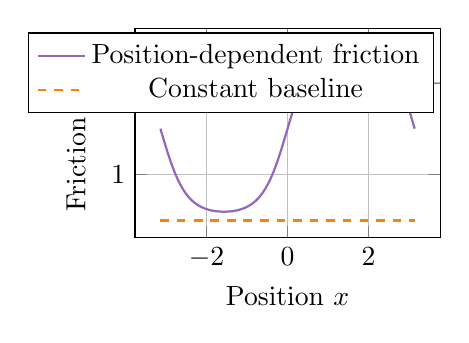
\begin{tikzpicture}
\begin{axis}[
    width=0.45\textwidth,
    height=0.35\textwidth,
    xlabel={Position $x$},
    ylabel={Friction $\mu(x)$},
    grid=major,
    domain=-pi:pi,
    samples=100,
]
\addplot[thermopurple, thick] {0.5 + 2/(1 + exp(-3*sin(deg(x))))};
\addlegendentry{Position-dependent friction}

\addplot[thermoorange, dashed, thick] {0.5};
\addlegendentry{Constant baseline}
\end{axis}
\end{tikzpicture}
\caption{\textbf{Left:} Velocity decay under different friction regimes. Low friction preserves momentum (blue), high friction quickly damps (red). \textbf{Right:} Position-dependent friction pattern, showing spatial variation in dissipative properties.}
\label{fig:friction-dynamics}
\end{figure}

Additionally, a learned gate $g(x) \in (0,1]$ scales the effective time step, implementing dynamic time scaling:

\begin{definition}[Dynamic Time Gate]
The effective time step is:
\[
\Delta t_{\text{eff}} = g(x) \cdot \Delta t,
\]
where $g(x)$ is a learned function of position (and optionally velocity).
\end{definition}

This gate implements:
\begin{itemize}
\item \textbf{Time contraction} ($g < 1$) in ``hard'' regions (high curvature), where small steps prevent overshooting.
\item \textbf{Time expansion} ($g \approx 1$) in ``flat'' regions, enabling skip-like behavior through large steps.
\end{itemize}

\begin{prop}[Time Gate Benefits]
\begin{enumerate}
\item \textbf{Numerical stability}: Smaller steps in high-curvature regions prevent integration failure.
\item \textbf{Computational efficiency}: Larger steps in flat regions skip redundant computation.
\item \textbf{Adaptive resolution}: The model allocates more computational resources to complex regions.
\end{enumerate}
\end{prop}

\section{Discrete-Time: Conformal Symplectic Leapfrog with Implicit Friction}

Implementing thermodynamic gating requires careful discretization to preserve the desired regime behavior.

\begin{definition}[Implicit Friction Leapfrog]
Let $\Delta t$ be the base step and $g(x) \in (0,1]$ the dynamic scale. Define $\Delta t_{\text{eff}} = g(x) \Delta t$ and $h = \frac{1}{2} \Delta t_{\text{eff}}$. A single leapfrog step with implicit friction is:

\begin{enumerate}
\item \textbf{Kick} (half step, implicit damping):
\[
v_{n+\frac{1}{2}} = \frac{v_n + h \cdot [F(x_n, u_n) - \Gamma(x_n, v_n)]}{1 + h \cdot \mu(x_n, u_n)}.
\]

\item \textbf{Drift} (full step position):
\[
x_{n+1} = \operatorname{wrap}\!\left(x_n + \Delta t_{\text{eff}} \cdot v_{n+\frac{1}{2}}\right).
\]

\item \textbf{Kick} (half step at new position):
\[
v_{n+1} = \frac{v_{n+\frac{1}{2}} + h \cdot [F(x_{n+1}, u_n) - \Gamma(x_{n+1}, v_{n+\frac{1}{2}})]}{1 + h \cdot \mu(x_{n+1}, u_n)}.
\]
\end{enumerate}
\end{definition}

The implicit form $\frac{v}{1 + h\mu}$ is crucial:

\begin{prop}[Implicit Friction Stability]
For the implicit update $v' = \frac{v + h \cdot a}{1 + h\mu}$, the magnitude satisfies:
\[
|v'| = \frac{|v + h \cdot a|}{\sqrt{(1 + h\mu)^2 + (h\mu)^2}} < |v + h \cdot a|,
\]
ensuring stability even for large $\mu$ values.
\end{prop}

This matches the reference implementation's fused CUDA/Python update and provides:

\begin{prop}[Leapfrog Properties]
\begin{enumerate}
\item \textbf{Conformal symplecticity}: Time-reversibility is broken only by $\mu$; when $\mu = 0$, the scheme is exactly symplectic.
\item \textbf{Localized energy transfer}: Energy production/consumption is confined to transitions, enabling ``dash-and-stop'' behavior.
\item \textbf{Dynamic time preservation}: The $g(x)$ gate preserves qualitative trajectories by shrinking steps near strong curvature.
\end{enumerate}
\end{prop}

\begin{remarque}[Periodic Topology]
The $\operatorname{wrap}(\cdot)$ function enforces toroidal topology by applying modulo $2\pi$ after position updates. This maintains coordinates on the manifold and prevents drift toward infinity.
\end{remarque}

\begin{figure}[htbp]
\centering
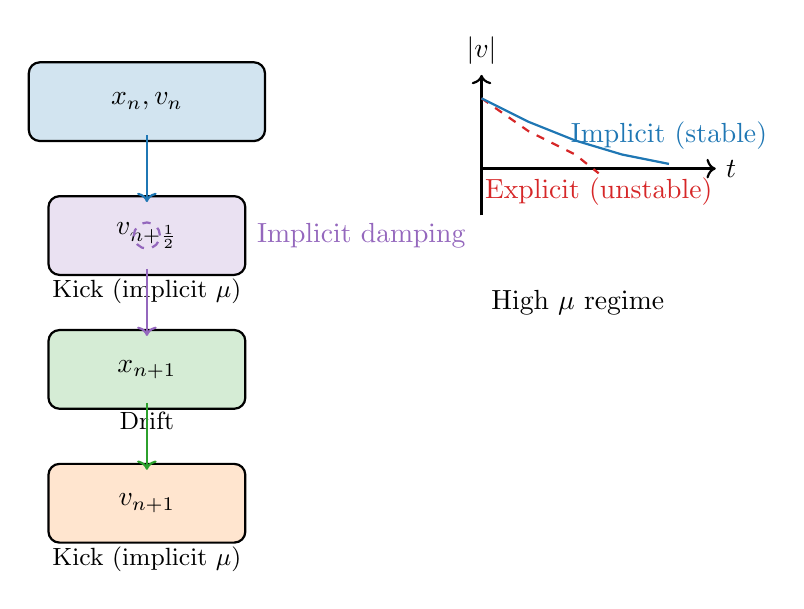
\begin{tikzpicture}[scale=0.85]
    % Leapfrog step visualization
    \node[draw, rectangle, rounded corners, fill=thermoblue!20, thick, minimum width=3cm, minimum height=1cm] at (0, 2) {$x_n, v_n$};
    
    \node[draw, rectangle, rounded corners, fill=thermopurple!20, thick, minimum width=2.5cm, minimum height=1cm] at (0, 0) {$v_{n+\frac{1}{2}}$};
    \node[below] at (0, -0.5) {\small Kick (implicit $\mu$)};
    
    \node[draw, rectangle, rounded corners, fill=thermogreen!20, thick, minimum width=2.5cm, minimum height=1cm] at (0, -2) {$x_{n+1}$};
    \node[below] at (0, -2.5) {\small Drift};
    
    \node[draw, rectangle, rounded corners, fill=thermoorange!20, thick, minimum width=2.5cm, minimum height=1cm] at (0, -4) {$v_{n+1}$};
    \node[below] at (0, -4.5) {\small Kick (implicit $\mu$)};
    
    % Arrows
    \draw[->, thick, thermoblue] (0, 1.5) -- (0, 0.5);
    \draw[->, thick, thermopurple] (0, -0.5) -- (0, -1.5);
    \draw[->, thick, thermogreen] (0, -2.5) -- (0, -3.5);
    
    % Friction effect visualization
    \begin{scope}[shift={(5, 1)}, scale=0.7]
        \draw[->, thick] (0, 0) -- (5, 0) node[right] {$t$};
        \draw[->, thick] (0, -1) -- (0, 2) node[above] {$|v|$};
        
        % Explicit Euler (unstable at high friction)
        \draw[thermored, dashed, thick] 
            plot coordinates {(0, 1.5) (1, 0.8) (2, 0.3) (2.5, -0.1)};
        \node[thermored] at (2.5, -0.5) {Explicit (unstable)};
        
        % Implicit (stable)
        \draw[thermoblue, thick] 
            plot coordinates {(0, 1.5) (1, 1.0) (2, 0.6) (3, 0.3) (4, 0.1)};
        \node[thermoblue, above] at (4, 0.2) {Implicit (stable)};
    \end{scope}
    
    % Annotations
    \node[right] at (5, -1) {High $\mu$ regime};
    \node[draw, ellipse, dashed, thermopurple, thick] at (0, 0) {};
    \node[thermopurple, right] at (1.5, 0) {Implicit damping};
\end{tikzpicture}
\caption{Left: Leapfrog step structure with implicit friction. Right: Comparison of explicit vs. implicit friction integration. Explicit methods become unstable at high friction, while implicit methods remain stable.}
\label{fig:leapfrog-implicit}
\end{figure}

\section{Implementation Summary}

The thermodynamic gating architecture consists of several interconnected components:

\subsection{Friction Gate (Thermodynamic Clutch)}

\begin{definition}[Friction Gate Architecture]
The friction coefficient is computed as:
\[
\mu(x,u) = \alpha \cdot \sigma\left(W_{\text{state}} \cdot \begin{bmatrix}\sin x \\ \cos x\end{bmatrix} + W_{\text{input}} \cdot u\right),
\]
where:
\begin{itemize}
\item $\alpha > 0$ is a learned maximum friction scale,
\item $\sigma(\cdot)$ is the sigmoid activation,
\item $[\sin x, \cos x]$ provides periodic features for toroidal manifolds,
\item $W_{\text{state}}$ and $W_{\text{input}}$ are learned projection matrices.
\end{itemize}
\end{definition}

On compact manifolds (torus), periodic features $[\sin x, \cos x]$ preserve continuity across $2\pi$ boundaries, preventing discontinuities in the gating function.

\subsection{Curvature Gate (Dynamic Time)}

\begin{definition}[Time Gate Architecture]
The dynamic time scale is:
\[
g(x) = \exp\left(-\theta \cdot \|W_g \cdot [\sin x, \cos x]\|\right) \in (0,1],
\]
where $\theta > 0$ controls the sensitivity to curvature.
\end{definition}

Alternatively, a small MLP can learn arbitrary time-scaling functions:
\[
g(x) = \sigma(\text{MLP}([\sin x, \cos x])).
\]

Both formulations respect periodicity through the input features.

\begin{prop}[Time Gate Behavior]
For regions of high curvature (large $\|\Gamma(x,v)\|$):
\begin{enumerate}
\item $g(x)$ decreases, contracting effective time.
\item Smaller steps prevent numerical instability.
\end{enumerate}
For flat regions:
\begin{enumerate}
\item $g(x) \approx 1$, allowing efficient large steps.
\end{enumerate}
\end{prop}

\subsection{Curvature Interaction}

The Christoffel-like curvature interaction is computed via a low-rank operator:
\[
\Gamma(x,v) = \sum_{r=1}^{R} \lambda_r \, (v^\top U_r) \, (U v)_r,
\]
with soft clamping for numerical safety:
\[
\Gamma_{\text{safe}} = \tanh\left(\frac{\Gamma}{C}\right) \cdot C.
\]

This symmetric structure approximates torsion-free geometry while remaining computationally efficient.

\begin{table}[htbp]
\centering
\begin{tabular}{lp{0.55\textwidth}}
\toprule
Component & Description \\
\midrule
\textbf{Friction Gate} & Linear mapping over periodic state features $[\sin x, \cos x]$ and optional input force; sigmoid activation bounds $\mu \in [0, \alpha]$. \\
\midrule
\textbf{Time Gate} & MLP or exponential decay over periodic features; $g(x) \in (0,1]$ scales $\Delta t$ per head. \\
\midrule
\textbf{Curvature} & Low-rank Christoffel approximation with soft clamping; symmetric structure for torsion-free geometry. \\
\midrule
\textbf{Integrator} & Leapfrog/Verlet/Yoshida/Forest-Ruth with implicit friction and periodic wrapping. \\
\midrule
\textbf{Multi-Head} & Latent state split across heads; each head applies independent geometry, gates, and integrator. \\
\bottomrule
\end{tabular}
\caption{Architecture components for thermodynamic gating.}
\label{tab:architecture}
\end{table}

\section{Topology and Periodic Features}

Thermodynamic gating is particularly effective on compact manifolds, especially toroidal topologies.

\begin{definition}[Toroidal Manifold]
The $n$-dimensional torus $T^n = (S^1)^n$ has:
\begin{itemize}
\item Local coordinates $x = (\theta_1, \ldots, \theta_n) \in [0, 2\pi)^n$.
\item Periodic boundary conditions $x \sim x + 2\pi k$ for $k \in \mathbb{Z}^n$.
\end{itemize}
\end{definition}

This topology is natural for modeling:

\begin{prop}[Natural Tasks for Toroidal Geometry]
\begin{enumerate}
\item \textbf{Parity tracking}: Binary states map to $\{\pi/2, 3\pi/2\}$.
\item \textbf{Phase tracking}: Continuous phases naturally wrap around $2\pi$.
\item \textbf{Modular arithmetic}: Addition modulo $N$ maps to phase addition.
\end{enumerate}
\end{prop}

Periodic features $[\sin x, \cos x]$ are used in both friction gating and time gating to preserve continuity:

\begin{remarque}[Feature Continuity]
Using $[\sin x, \cos x]$ instead of $x$ ensures:
\begin{itemize}
\item Smooth gradients at boundaries $x = 0$ and $x = 2\pi$.
\item Translation invariance under wrapping.
\end{itemize}
This is essential for stable training on toroidal manifolds.
\end{remarque}

\begin{figure}[htbp]
\centering
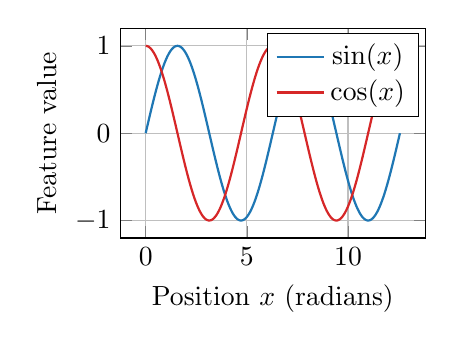
\begin{tikzpicture}
\begin{axis}[
    width=0.45\textwidth,
    height=0.35\textwidth,
    xlabel={Position $x$ (radians)},
    ylabel={Feature value},
    grid=major,
    domain=0:4*pi,
    samples=200,
]
\addplot[thermoblue, thick] {sin(deg(x))};
\addlegendentry{$\sin(x)$}

\addplot[thermored, thick] {cos(deg(x))};
\addlegendentry{$\cos(x)$}
\end{axis}
\end{tikzpicture}
\hfill
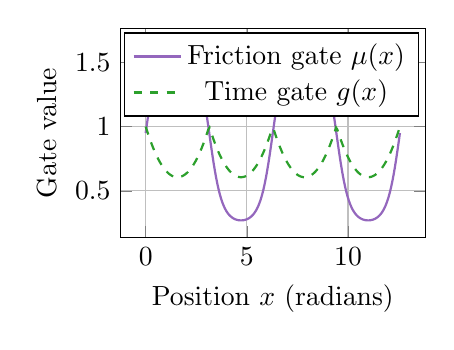
\begin{tikzpicture}
\begin{axis}[
    width=0.45\textwidth,
    height=0.35\textwidth,
    xlabel={Position $x$ (radians)},
    ylabel={Gate value},
    grid=major,
    domain=0:4*pi,
    samples=200,
]
\addplot[thermopurple, thick] {0.2 + 1.5/(1 + exp(-3*sin(deg(x))))};
\addlegendentry{Friction gate $\mu(x)$}

\addplot[thermogreen, dashed, thick] {exp(-0.5*abs(sin(deg(x))))};
\addlegendentry{Time gate $g(x)$}
\end{axis}
\end{tikzpicture}
\caption{\textbf{Left:} Periodic features $[\sin x, \cos x]$ provide smooth, continuous representations on the torus. \textbf{Right:} Resulting gate values showing periodic variation respecting the manifold topology.}
\label{fig:periodic-features}
\end{figure}

Position updates apply $\operatorname{wrap}(\cdot)$ to maintain coordinates on the manifold:
\[
\operatorname{wrap}(x) = x - 2\pi \left\lfloor \frac{x}{2\pi} + \frac{1}{2} \right\rfloor.
\]

Training losses include toroidal distance terms to avoid boundary artifacts:
\[
L_{\text{torus}} = \min\left(|\Delta|, 2\pi - |\Delta|\right)^2.
\]

\section{Training and Regularization}

Training thermodynamic gating models requires balancing multiple objectives.

\begin{definition}[Total Loss]
\[
L = L_{\text{task}} + \lambda_H L_H + \lambda_\Gamma L_\Gamma + \lambda_{\text{vel}} L_{\text{vel}},
\]
where $\lambda_H, \lambda_\Gamma, \lambda_{\text{vel}}$ are balancing coefficients.
\end{definition}

\subsection{Task Losses}

For different output types:

\begin{prop}[Task Loss Selection]
\begin{itemize}
\item \textbf{Classification}: Cross-entropy on output logits.
\item \textbf{Continuous periodic}: Toroidal distance loss $L_{\text{torus}}$.
\item \textbf{Phase regression}: Bounded phase loss $L_{\text{phase}} = 1 - \cos(\Delta)$.
\end{itemize}
\end{prop}

\subsection{Hamiltonian Stability}

To prevent spurious energy creation during coasting:
\[
L_H = \mathbb{E}\left[|E_{t+1} - E_t|\right], \quad E_t = \frac{1}{2}v_t^\top g(x_t) v_t.
\]
This encourages conservative dynamics when $\mu \approx 0$.

\subsection{Geodesic Regularization}

To encourage curvature smoothness:
\[
L_\Gamma = \mathbb{E}\left[\|\Gamma(x_t, v_t)\|^2\right].
\]
This reduces instability under strong gates.

\subsection{Velocity Saturation}

To limit runaway speeds:
\[
L_{\text{vel}} = \mathbb{E}\left[\tanh^{-1}\left(\min\left(\frac{\|v\|}{V_{\max}}, 0.99\right)\right)\right].
\]
This keeps gradients well-behaved while allowing large velocities when needed.

\begin{remarque}[Regularization Balance]
The coefficients $\lambda_H, \lambda_\Gamma, \lambda_{\text{vel}}$ must be tuned for each task. Too much Hamiltonian regularization prevents useful dissipation; too little causes instability.
\end{remarque}

\section{Information-Theoretic Perspective}

Thermodynamic gating realizes \textbf{Landauer's Principle}: erasure requires dissipating energy.

\begin{definition}[Landauer's Principle]
Erasing one bit of information requires minimum energy dissipation:
\[
\Delta E \geq k_B T \ln 2,
\]
where $k_B$ is Boltzmann's constant and $T$ is temperature.
\end{definition}

In our model:
\begin{itemize}
\item \textbf{Low dissipation} ($\mu \approx 0$): Information is conserved, not erased---no thermodynamic cost.
\item \textbf{High dissipation} ($\mu \gg 0$): Information is actively erased, requiring energy dissipation proportional to the magnitude of rewriting.
\end{itemize}

Trained models exhibit:

\begin{prop}[Learned Gating Behavior]
\begin{enumerate}
\item \textbf{Low dissipation during stationary contexts}: Memory conservation when no rewriting is needed.
\item \textbf{Sharp $\mu$ spikes at transitions}: Entropy production precisely where semantic changes occur.
\item \textbf{Time contraction near complex geometry}: Avoiding aliasing in regions requiring fine-grained processing.
\end{enumerate}
\end{prop}

This yields precise state changes without sacrificing long-horizon persistence—the best of both worlds.

\begin{figure}[htbp]
\centering
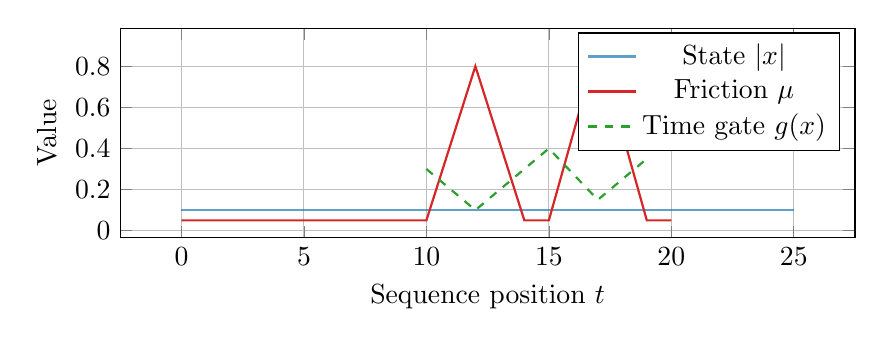
\begin{tikzpicture}
\begin{axis}[
    width=0.9\textwidth,
    height=0.35\textwidth,
    xlabel={Sequence position $t$},
    ylabel={Value},
    grid=major,
    samples=150,
]
\addplot[thermoblue, thick, opacity=0.7] coordinates {
    (0, 0.1) (5, 0.1) (10, 0.1) (15, 0.1) (20, 0.1) (25, 0.1)
};
\addlegendentry{State $|x|$}

\addplot[thermored, thick] coordinates {
    (0, 0.05) (5, 0.05) (10, 0.05) (12, 0.8) (14, 0.05) (15, 0.05) (17, 0.9) (19, 0.05) (20, 0.05)
};
\addlegendentry{Friction $\mu$}

\addplot[thermogreen, dashed, thick] coordinates {
    (10, 0.3) (12, 0.1) (14, 0.3) (15, 0.4) (17, 0.15) (19, 0.35)
};
\addlegendentry{Time gate $g(x)$}
\end{axis}
\end{tikzpicture}
\caption{Information-theoretic behavior during sequence processing. The state (blue) remains stable during stationary contexts. At semantic transitions (around $t=12, 17$), friction $\mu$ spikes (red), implementing thermodynamic erasure. The time gate $g(x)$ (green) contracts during transitions.}
\label{fig:information-flow}
\end{figure}

This perspective connects neural computation to physical laws, suggesting that optimal gating policies naturally emerge from the need to balance information preservation against necessary rewriting.

\section{Practical Notes}

Several implementation details ensure stability and efficiency:

\begin{remarque}[Stability Guidelines]
\begin{enumerate}
\item \textbf{Bound maximum friction}: $\mu_{\max}$ is bounded to maintain stability under implicit updates.
\item \textbf{Per-head and per-batch gates}: Enable heterogeneous regimes across manifold subspaces.
\item \textbf{CUDA fused paths}: Accelerate integration and gating for training throughput.
\item \textbf{Python fallbacks}: Preserve correctness where fused kernels are unavailable.
\end{enumerate}
\end{remarque}

The toroidal wrapping is applied after position updates:
\[
x_{t+1} = \operatorname{wrap}(x_t + \Delta t_{\text{eff}} \cdot v_{t+\frac{1}{2}}).
\]

Gating features remain periodic to avoid discontinuities at boundaries. The combination ensures stable, efficient computation across all operating regimes.

\section{Conclusion}

Thermodynamic Gating unifies conservative memory and decisive updating within a single geometric computation layer:

\begin{prop}[Key Contributions]
\begin{enumerate}
\item \textbf{Physical grounding}: Dissipation connects to thermodynamic principles (Landauer's principle).
\item \textbf{Regime control}: The same architecture handles both persistent memory (coasting) and rapid rewriting (damping).
\item \textbf{Stability}: Implicit friction discretization prevents instability even at high dissipation.
\item \textbf{Efficiency}: Dynamic time gating allocates computation where needed.
\end{enumerate}
\end{prop}

By combining a conformal-symplectic integrator with learned friction and dynamic time gating, Geodesic Flow Networks achieve:

\begin{itemize}
\item \textbf{Stability}: Phase-space volume preservation when needed.
\item \textbf{Persistence}: Long-horizon memory along geodesics.
\item \textbf{Controllability}: Precise state changes at semantic transitions.
\end{itemize}

This enables symbolic trajectory formation and robust reasoning over long horizons, connecting deep learning to fundamental physical principles.

\clearpage

\appendix

\section{Derivation of Implicit Friction Update}

Starting from the continuous dynamics:
\[
\dot{v} = F - \Gamma - \mu v.
\]

Discretizing with step size $h = \Delta t / 2$:

\[
\frac{v_{n+1} - v_n}{h} = F_n - \Gamma_n - \mu_n \frac{v_{n+1} + v_n}{2}.
\]

Solving for $v_{n+1}$:

\begin{align}
v_{n+1} - v_n &= h F_n - h \Gamma_n - \frac{h \mu_n}{2} (v_{n+1} + v_n) \\
v_{n+1} + \frac{h \mu_n}{2} v_{n+1} &= v_n + h F_n - h \Gamma_n - \frac{h \mu_n}{2} v_n \\
v_{n+1} \left(1 + \frac{h \mu_n}{2}\right) &= v_n \left(1 - \frac{h \mu_n}{2}\right) + h(F_n - \Gamma_n) \\
v_{n+1} &= \frac{v_n + h(F_n - \Gamma_n)}{1 + h \mu_n}.
\end{align}

This yields the implicit friction update used in the leapfrog step.

\section{Implementation Code}

\begin{minted}[mathescape, fontsize=\small, frame=lines]{python}
import jax.numpy as jnp
from jax import jit, nn

class ThermodynamicGating:
    def __init__(self, d_model=64, alpha=1.0, theta=0.5):
        self.d_model = d_model
        self.alpha = alpha  # Maximum friction
        self.theta = theta  # Time gate sensitivity
        
        # Friction gate parameters
        self.W_friction = jnp.randn(d_model, 2) * 0.1
        
        # Time gate parameters
        self.W_time = jnp.randn(d_model, 2) * 0.1
        
        # Curvature parameters (low-rank)
        self.rank = 8
        self.U = jnp.randn(d_model, self.rank) / jnp.sqrt(self.rank)
        self.lambda_r = jnp.randn(self.rank) * 0.1
        
        # Force projection
        self.W_force = jnp.randn(d_model, d_model) * 0.1
        
    def periodic_features(self, x):
        """Compute periodic features for toroidal manifolds."""
        return jnp.concatenate([jnp.sin(x), jnp.cos(x)], axis=-1)
    
    def friction_gate(self, x, u):
        """Compute state- and input-dependent friction."""
        features = self.periodic_features(x)
        gate_input = jnp.dot(features, self.W_friction)
        return nn.sigmoid(gate_input) * self.alpha
    
    def time_gate(self, x):
        """Compute dynamic time scale."""
        features = self.periodic_features(x)
        magnitude = jnp.linalg.norm(jnp.dot(features, self.W_time))
        return jnp.exp(-self.theta * magnitude)
    
    def curvature(self, x, v):
        """Compute Christoffel-like curvature interaction."""
        p = jnp.einsum('ij,kj->ik', v, self.U)
        Gamma = jnp.einsum('r,ir,jr->ij', self.lambda_r, p, p)
        # Soft clamping
        return jnp.tanh(Gamma / 5.0) * 5.0
    
    def force(self, x, u):
        """Compute token-driven force."""
        return jnp.dot(u, self.W_force.T)
    
    def effective_acceleration(self, x, v, u):
        """Compute full acceleration with friction."""
        F = self.force(x, u)
        Gamma = self.curvature(x, v)
        mu = self.friction_gate(x, u)
        
        return F - jnp.einsum('ij,j->i', Gamma, v) - mu * v
    
    @jit
    def leapfrog_step(self, x, v, u, dt=0.1):
        """Implicit friction leapfrog step."""
        # Dynamic time scaling
        g = self.time_gate(x)
        dt_eff = g * dt
        h = 0.5 * dt_eff
        
        # Kick (implicit friction)
        a = self.effective_acceleration(x, v, u)
        mu = self.friction_gate(x, u)
        v_half = (v + h * a) / (1 + h * mu)
        
        # Drift (with wrapping)
        x_new = (x + dt_eff * v_half) % (2 * jnp.pi)
        
        # Kick at new position
        a_new = self.effective_acceleration(x_new, v_half, u)
        mu_new = self.friction_gate(x_new, u)
        v_new = (v_half + h * a_new) / (1 + h * mu_new)
        
        return x_new, v_new
    
    def energy(self, x, v):
        """Compute kinetic energy under metric."""
        return 0.5 * jnp.sum(v ** 2)
\end{minted}

\section{Phase-Space Volume Analysis}

For the dissipative dynamics $\dot{v} = -\mu v$, the phase-space volume contracts:

\begin{prop}[Liouville's Theorem Modification]
The phase-space volume evolution follows:
\[
\frac{d}{dt} \log(\det D\Phi_t) = -\int \mu(x,u) \, \diff x.
\]
This is negative when $\mu > 0$, confirming entropy production.
\end{prop}

In contrast, conservative dynamics ($\mu = 0$) preserve phase-space volume exactly:
\[
\frac{d}{dt} \log(\det D\Phi_t) = 0.
\]

This dichotomy---volume preservation vs. contraction---is the geometric manifestation of the memory/update trade-off.

\end{document}
